\section{Deterministic electricity market clearing problem} \label{sec:deter}
In this section, we introduce the deterministic electricity market clearing problem. The primary linear programming problem is first presented, followed by its dual problem. The KKT optimality conditions are also derived.
\subsection{Primary problem}
The primary market clearing problem considering network is expanded as follows, where the objective function (\ref{1.obj}) is minimizing the overall cost. (\ref{1.production}) constrains each generator's production within their own capacity. (\ref{1.wind}) shows that wind power dispatch is limited by its predicted output, where $CF$ is the predicted capacity factor. The power balance for each node is represented with (\ref{1.balance}), where $\lambda_n$ are the locational marginal prices. The power flow limits within transmission lines are shown in (\ref{1.flow}). (\ref{1.ref}) states the voltage angle of the reference bus.
\begin{subequations}
\begin{equation} \label{1.obj}
\underset{p_{g}^{G}, P_w^W, \theta_{n}} \min \sum_{g} C_{g} p_{g}^{\mathrm{G}}
\end{equation}
% \begin{equation}\label{1.demand}
% 0 \leq p_{d}^{\mathrm{D}} \leq \bar{P}_{d}^{\mathrm{D}}: \underline{\mu}_{d}^{\mathrm{D}}, \bar{\mu}_{d}^{\mathrm{D}} \quad \forall d
% \end{equation}
\begin{equation}\label{1.production}
\text{S.t.} \quad \quad
 0 \leq p_{g}^{\mathrm{G}} \leq {P}_{g}^{max}: \underline{\mu}_{g}^{\mathrm{G}}, \bar{\mu}_{g}^{\mathrm{G}} \quad \forall g
\end{equation}
\begin{equation} \label{1.wind}
   0 \leq p_w^W \leq P_w^{Cap} CF_w :\underline{\mu}_{w}^{\mathrm{W}}, \bar{\mu}_{w}^{\mathrm{W}} \quad \forall w
\end{equation}
\begin{equation}\label{1.balance}
\sum_{d \in \Psi_{n}} p_{d}^{\mathrm{D}}+\sum_{m \in \Omega_{n}} B_{n, m}\left(\theta_{n}-\theta_{m}\right)-\sum_{g \in \Psi_{n}} p_{g}^{\mathrm{G}} - \sum_{w \in \Psi_{n}} p_{w}^{\mathrm{W}} =0 \quad: \lambda_{n} \quad \forall n
\end{equation}
\begin{equation}\label{1.flow}
-F_{n, m} \leq B_{n, m}\left(\theta_{n}-\theta_{m}\right) \leq F_{n, m} \quad: \underline{\eta}_{n, m}, \bar{\eta}_{n, m} \quad \forall n, \forall m 
\end{equation}
\begin{equation}\label{1.ref}
\theta_{(n=r e f)}=0 \quad: \gamma
\end{equation}
\end{subequations}

\subsection{Dual problem}

In order to derive the dual problem, we need to write the Lagrangian function. For clarity, we use vectors $\boldsymbol{\mu}$ to represent the dual variables of (\ref{1.production})(\ref{1.wind}), $\boldsymbol{\lambda}$ for (\ref{1.balance}) and  $\boldsymbol{\eta}$ for (\ref{1.flow}). Then we can write the Lagrangian function as follows.
\begin{equation}
\begin{split}
    L(p_{g}^{G}, p_w^W, \theta_{n}, \boldsymbol{\mu},\boldsymbol{\lambda}, \boldsymbol{\eta}, \gamma) = \sum_{g} C_{g} p_{g}^{\mathrm{G}} + \sum_{g} \bar{\mu}_{g}^{\mathrm{G}}(p_{g}^{\mathrm{G}}-P_g^{max}) - \sum_{g}\underline{\mu}_{g}p_{g}^{\mathrm{G}} +\sum_w\bar{\mu}_w^W(p_w^W-P_w^{Cap}CF_w) \\ - \sum_w\underline{\mu}_w^W p_w^W + \sum_n \lambda_{n}(\sum_{d \in \Psi_{n}} p_{d}^{\mathrm{D}}+\sum_{m \in \Omega_{n}} B_{n, m}\left(\theta_{n}-\theta_{m}\right)-\sum_{g \in \Psi_{n}} p_{g}^{\mathrm{G}}- \sum_{w \in \Psi_{n}} p_{w}^{\mathrm{W}})\\+ \sum_{n, m} \bar{\eta}_{n, m}(B_{n, m}\left(\theta_{n}-\theta_{m}\right)-F_{n,m}) -\sum_{n, m} \underline{\eta}_{n, m}(B_{n, m}\left(\theta_{n}-\theta_{m}\right)+F_{n,m}) + \gamma \theta_{(n=r e f)}
\end{split}
\end{equation}

Then the dual function can be expressed as:
\begin{equation}
    g(\boldsymbol{\mu},\boldsymbol{\lambda}, \boldsymbol{\eta}, \gamma) = \underset{p_{g}^{G}, p_w^W, \theta_{n}} \min L(p_{g}^{G}, p_w^W, \theta_{n}, \boldsymbol{\mu},\boldsymbol{\lambda}, \boldsymbol{\eta}, \gamma) 
\end{equation}

The dual problem is then:
\begin{equation} \label{1.dualProblem}
    \underset{\boldsymbol{\mu}\geq\boldsymbol{0},\boldsymbol{\lambda}, \boldsymbol{\eta}\geq\boldsymbol{0}, \gamma}{\max}g(\boldsymbol{\mu},\boldsymbol{\lambda}, \boldsymbol{\eta}, \gamma) =     \underset{\boldsymbol{\mu}\geq\boldsymbol{0},\boldsymbol{\lambda}, \boldsymbol{\eta}\geq\boldsymbol{0}, \gamma}{\max} \left\{ \underset{p_{g}^{G}, p_w^W, \theta_{n}} \min L(p_{g}^{G}, p_w^W, \theta_{n}, \boldsymbol{\mu},\boldsymbol{\lambda}, \boldsymbol{\eta}, \gamma)  \right\}
\end{equation}

The above max-min problem can be reformulated by taking the KKT conditions of the inner minimization problem and moving the objective function out, which gives us:
% The above max-min optimization problem can also be formulated as:
% \begin{subequations}
% \begin{equation}
%  \underset{\boldsymbol{\mu}\geq\boldsymbol{0},\boldsymbol{\lambda}, \boldsymbol{\eta}\geq\boldsymbol{0}, \gamma}{\max}\sum_{d}\bar{\mu}_{d}^{\mathrm{D}}(-\bar{P}_{d}^{\mathrm{D}}) + \sum_{g}\bar{\mu}_{g}^{\mathrm{G}}(-\bar{P}_{g}^{\mathrm{G}}) - \sum_{n, m} \bar{\eta}_{n, m} F_{n,m} - \sum_{n, m} \underline{\eta}_{n, m} F_{n,m}
% \end{equation}
% \begin{equation}
%     \textbf{s.t.} \quad  \text{KKT conditions of (\ref{1.dualProblem})'s inner optimization problem}
% \end{equation}
% \end{subequations}

% As (\ref{1.dualProblem})'s inner optimization problem has no constraints, its KKT conditions can be derived by taking the partial derivatives of the Lagrangian function with respect to each variable as 0. The dual problem is listed as 
\begin{subequations} 
\begin{equation}\label{1.dualOBJ}
\underset{\boldsymbol{\mu}\geq\boldsymbol{0},\boldsymbol{\lambda}, \boldsymbol{\eta}\geq\boldsymbol{0}, \gamma}{\min} \sum_{g}\bar{\mu}_{g}^{\mathrm{G}}P_g^{max} + \sum_w\bar{\mu}_w^W P_w^{Cap}CF_w - \sum_n\lambda_n\sum_{d \in \Psi_n}P_d^D  + \sum_{n, m} \bar{\eta}_{n, m} F_{n,m} +\sum_{n, m} \underline{\eta}_{n, m} F_{n,m}
\end{equation}
\begin{equation} \label{6b}
    C_g + \bar{\mu}_g^G - \underline{\mu}_g^G - \lambda_{n(g \in \Psi_{n})} = 0 \quad:p_g^G, \forall g
\end{equation}
\begin{equation} \label{6c}
\bar{\mu}_w^W - \underline{\mu}_w^W - \lambda_{n(w\in\Psi_n)} = 0 \quad:p_w^W, \forall w
\end{equation}
\begin{equation} \label{6d}
\sum_{m \in \Omega_n}B_{n,m}(\lambda_n - \lambda_m + \bar{\eta}_{n,m}-\bar{\eta}_{m,n}-\underline{\eta}_{n,m}+\underline{\eta}_{m,n}) = 0 \quad: \theta_n, \forall n/ref
\end{equation}
\begin{equation}\label{6e}
\sum_{m \in \Omega_n}B_{n,m}(\lambda_n - \lambda_m + \bar{\eta}_{n,m}-\bar{\eta}_{m,n}-\underline{\eta}_{n,m}+\underline{\eta}_{m,n})+\gamma = 0 \quad: \theta_n, n=ref
\end{equation}


Alternatively, by eliminating non-negative variables $\underline{\mu}_g^G$ and $\underline{\mu}_w^W$, constraints (\ref{6b}) and (\ref{6c}) can be replaced with (\ref{new6b}) and (\ref{new6c}). Then (\ref{1.dualOBJ}) and (\ref{6d})-(\ref{new6c}) give the dual optimization problem.

\begin{equation} \label{new6b}
    C_g + \bar{\mu}_g^G - \lambda_{n(g \in \Psi_{n})} \geq 0 \quad:p_g^G, \forall g
\end{equation}
\begin{equation} \label{new6c}
\bar{\mu}_w^W - \lambda_{n(w\in\Psi_n)} \geq 0 \quad:p_w^W, \forall w
\end{equation}
\end{subequations}

\subsection{KKT conditions of primary problem}
The KKT conditions include three different sets of constraints. (\ref{6b})-(\ref{6e}) give the set with respect to partial derivatives. (\ref{1.balance}) and (\ref{1.ref}) keeps the same as primary feasible conditions. Following conditions (\ref{kkt1})-(\ref{kkt6}) represent as the complementary slackness conditions. Overall, (\ref{6b})-(\ref{6e}), (\ref{1.balance})-(\ref{1.ref}) and (\ref{kkt1})-(\ref{kkt6}) give the KKT conditions for the primary problem, where $\boldsymbol{\lambda}$ and $\gamma$ are free variables.

\begin{subequations}
\begin{equation}\label{kkt1}
    0 \leq p_g^G \perp \underline{\mu}_g^G \geq 0, \forall g
\end{equation}
\begin{equation}\label{kkt2}
    0 \geq (p_g^G - P_g^{max}) \perp \bar{\mu}_g^G \geq 0, \forall g
\end{equation}
\begin{equation}\label{kkt3}
    0 \leq p_w^W \perp \underline{\mu}_w^W \geq 0, \forall w
\end{equation}
\begin{equation}\label{kkt4}
    0 \geq (p_w^W - P_w^{Cap}CF_w) \perp \bar{\mu}_w^W \geq 0, \forall g
\end{equation}
\begin{equation}\label{kkt5}
  0\leq [B_{n,m}(\theta_n - \theta_m)+F_{n,m}] \perp \underline{\eta}_{n,m} \geq 0, \forall n, \forall m
\end{equation}
\begin{equation}\label{kkt6}
  0\geq [B_{n,m}(\theta_n - \theta_m)-F_{n,m}] \perp \bar{\eta}_{n,m} \geq 0, \forall n, \forall m
\end{equation}
\end{subequations}

In order to solve the KKT conditions, a trivial objective function is set, such as 0. The complementary slackness constraints can be linearized using "big M" method, where M is an arbitrarily large parameter. Then (\ref{kkt1})-(\ref{kkt6}) can be replaced with (\ref{bigm3})-(\ref{bigm6}).
\begin{subequations}
\begin{equation}\label{bigm3}
    0\leq p_g^G \leq M\delta_{g,1},\quad 0\leq \underline{\mu}_g^G \leq M\delta_{g,2}, \quad \delta_{g,1}+\delta_{g,2} \leq 1, \forall g
\end{equation}
\begin{equation}\label{bigm4}
    0\leq {P}_g^{max} - p_g^G \leq M\delta_{g,3},\quad 0\leq \bar{\mu}_g^G \leq M\delta_{g,4}, \quad \delta_{g,3}+\delta_{g,4} \leq 1, \forall g
\end{equation}
\begin{equation} \label{bigm1}
    0\leq p_w^W \leq M\delta_{w,1},\quad 0\leq \underline{\mu}_w^W \leq M\delta_{w,2}, \quad \delta_{w,1}+\delta_{w,2} \leq 1, \forall w
\end{equation}
\begin{equation}\label{bigm2}
    0\leq P_w^{Cap}CF_w - P_w^W \leq M\delta_{w,3},\quad 0\leq \bar{\mu}_w^W \leq M\delta_{w,4}, \quad \delta_{w,3}+\delta_{w,4} \leq 1, \forall w
\end{equation}
\begin{equation}\label{bigm5}
    0\leq [B_{n,m}(\theta_n - \theta_m)+F_{n,m}] \leq M\delta^1_{n,m}, 0 \leq \underline{\eta}_{n,m} \leq M\delta^2_{n,m}, \delta^1_{n,m}+\delta^2_{n,m} \leq 1, \forall n, \forall m
\end{equation}
\begin{equation}\label{bigm6}
    0\leq [F_{n,m}-B_{n,m}(\theta_n - \theta_m)] \leq M\delta^3_{n,m}, 0 \leq \bar{\eta}_{n,m} \leq M\delta^4_{n,m}, \delta^3_{n,m}+\delta^4_{n,m} \leq 1, \forall n, \forall m
\end{equation}
\end{subequations}

\subsection{Case study}
The LP and mixed integer linear programming (MILP) problems are formulated with JuMP package on Julia solved with Gurobi solver. As expected, the primary, dual problem and KKT conditions generate exactly the same result in terms of power generation and nodal prices. In our case, setting the big number M as 5,000 gives reasonable results. If M goes up to 10,000, the complementarity conditions no longer hold.

\begin{figure}[h]
    \centering
    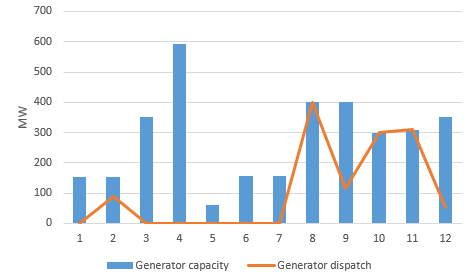
\includegraphics{figures/1generatordispatch.png}
    \caption{Generator dispatch}
    \label{fig:1.generator}
\end{figure}

\begin{figure}[h]
    \centering
    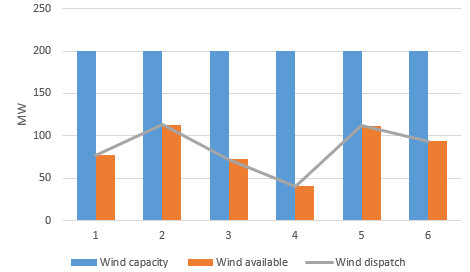
\includegraphics{figures/1winddispatch.png}
    \caption{Wind dispatch}
    \label{fig:1.wind}
\end{figure}

The minimized social cost is \$8,063, as a result of a high penetration of wind power with a generation cost of 0. From fig. \ref{fig:1.generator}, generator units 8, 10 and 11 are fully dispatched, while generator 1, 3, 4, 5, 6 and 7 are not dispatched, as results of its relatively higher offering price against wind generators and other generators. Fig. \ref{fig:1.wind} indicates that all the available wind power are dispatched, due to its zero marginal price.

The locational marginal prices (LMPs) are reported on tab. \ref{tab:1lmp} for each node. The prices are generally different but close, which might be resulting from price multiplicity.

\begin{table}[h]
    \centering
    \begin{tabular}{|c|c|c|c|c|c|c|c|c|}
    \hline
      \textbf{Node}   &  1 & 2 & 3& 4& 5& 6& 7 & 8\\
      \hline
        \textbf{LMP(\$/MWh)} & 13.28&13.32&11.93&13.45&13.56&13.72&13.70&13.70\\
        \hline
        \textbf{Node} & 9 &10&11&12&13&14&15&16\\
        \hline
        \textbf{LMP(\$/MWh)} & 13.55 & 13.85&   15.13 &  13.06&   13.40 &  18.08&   9.35 &  8.12\\
                \hline
        \textbf{Node} &17&18&19&20&21&22&23&24\\
        \hline
        \textbf{LMP(\$/MWh)} & 6.73 & 6.07  &9.30&  10.32 & 5.47&  5.96 & 10.89 & 10.35\\
        \hline
    \end{tabular}
    \caption{LMP for each node}
    \label{tab:1lmp}
\end{table}

% The LMPs are generally not the same for each node, which however, is not due to any line congestion. In fact, no line has experienced congestion in this case. One assumption is that with the constraint (\ref{1.balance}), all the power flow between nodes are correlated. Suppose node 1 has the reference voltage angle, in order to increase the power flow from node 1 to node 2, the voltage angle of node 2 has to decrease, which in return, changes all the power flow between node 2 and other nodes. In order to examine this assumption, we remove the voltage angle variables in the primary problem. Instead, new power flow variables are introduced, with only the line capacity constraints. In this way, power flow between different cables are not correlated. It turns out that in this case, the LMPs are either 6.02 or 10.52 $\$/MWh$. This actually corresponds to the argument that nodes with free power flow have equal LMPs. Therefore, the made assumption might be reasonable.

